\chapter{Detector Applications to measuring the active brain}
Lorem ipsum dolor sit amet, consectetur adipiscing elit. Nulla ligula lorem, malesuada non feugiat a, bibendum sit amet leo. Sed in dui lacus. Nullam quam dolor, elementum ac semper vitae, lacinia et dui. Curabitur accumsan urna nec dolor porttitor mollis. Nunc id feugiat tellus. Proin orci arcu, egestas a tincidunt eu, luctus ut ligula. Curabitur at risus non nulla congue facilisis sed eu velit. Morbi eget bibendum sem.

Cras vel lectus leo. Donec at ante vel eros condimentum dignissim et at libero. Nullam vitae purus at diam semper gravida. Ut venenatis dapibus nulla pretium eleifend. Nam scelerisque dignissim augue, ac suscipit tellus vestibulum vel. Sed rutrum sollicitudin sodales. Pellentesque cursus lobortis neque, id ornare purus laoreet eget. Sed adipiscing sollicitudin convallis. Quisque eu orci sit amet libero mollis tincidunt. Nullam sed consectetur odio. Etiam a molestie orci.

\section{{F}unctional {N}ear-{I}nfrared {fNIR} Imaging}
% detector applicaitons to improving fNIR
\begin{figure}[b]
  \begin{center}
    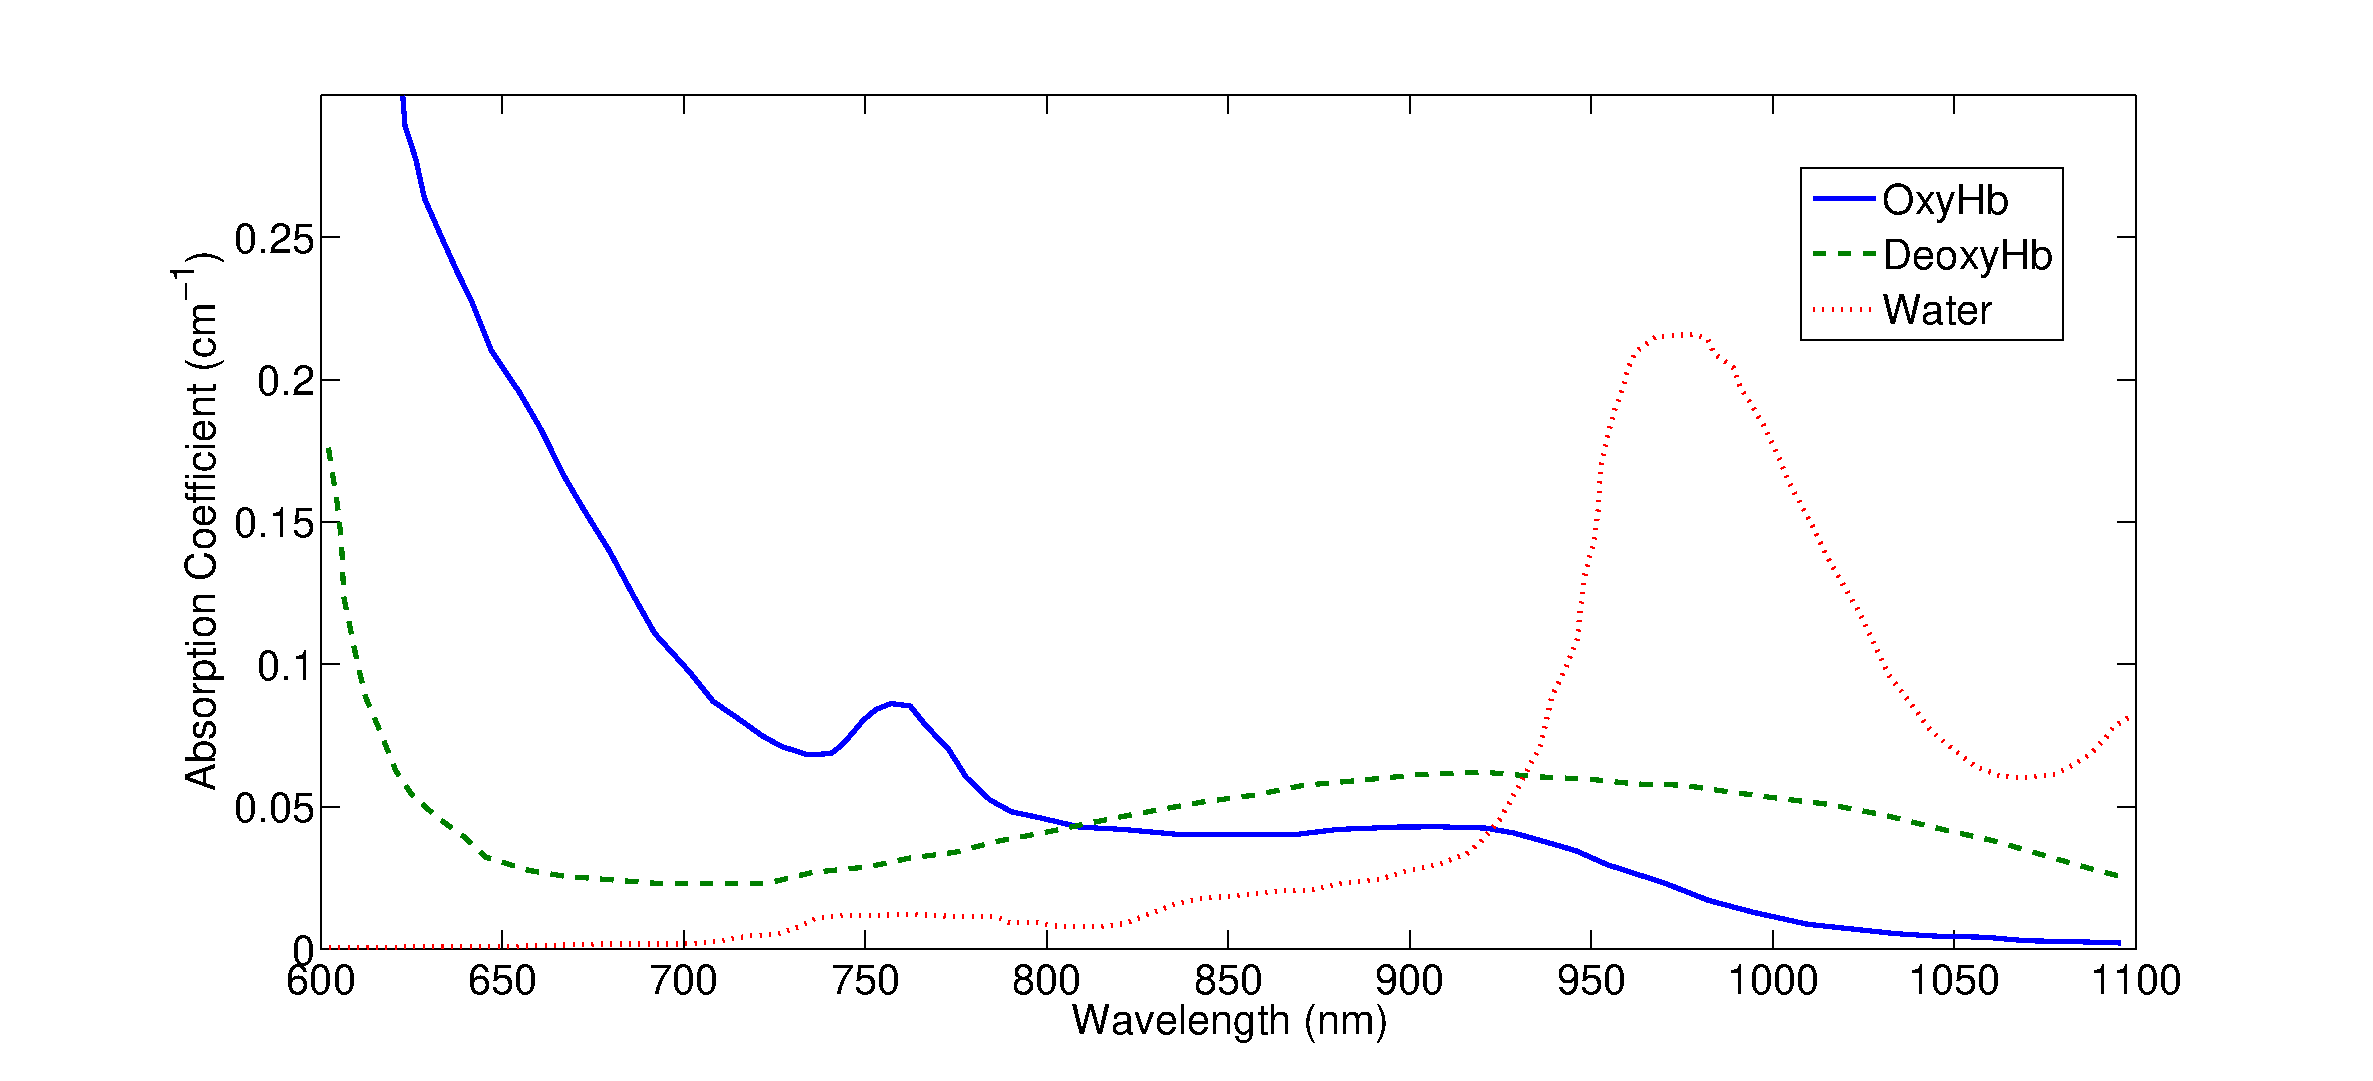
\includegraphics{AbsorptionData}
    \caption[Absorption spectra of water, deoxyhemoglobin and oxyhemoblogin]{\label{fig:fnirabsorption} Absorption spectra of water, Hb and Dhb.  From \citet{cope} and HB stuff from \citet{horecker} }
  \end{center}
\end{figure}

As discussed in previous sections, changes in tissue activity can be detected by measuring the change in blood oxygenation levels.  Functional Magnetic Resonance Imaging (fMRI) is one technique for accomplishing this (through measuring the BOLD response), but other techniques exist.  

The blood oxygenation can be determined by measuring the relative concentrations of oxyhemoglobin (oxy-Hb) and deoxyhemoglobin (deoxy-Hb).  Since oxy-Hb and deoxy-Hb have different absorption spectra (\cref{fig:fnirabsorption}), it is possible to determine this through optical techniques.

\begin{align}
  \label{eq:o2bloodvolume}
  Oxygenation\ &= \Delta C_{HBO2} - \Delta C_{HB} \nonumber \\
  Blood\ Volume\ &= \Delta C_{HBO2} + \Delta C_{HB} 
\end{align}

Lorem ipsum dolor sit amet, consectetur adipiscing elit. Nulla ligula lorem, malesuada non feugiat a, bibendum sit amet leo. Sed in dui lacus. Nullam quam dolor, elementum ac semper vitae, lacinia et dui. Curabitur accumsan urna nec dolor porttitor mollis. Nunc id feugiat tellus. Proin orci arcu, egestas a tincidunt eu, luctus ut ligula. Curabitur at risus non nulla congue facilisis sed eu velit. Morbi eget bibendum sem.

Cras vel lectus leo. Donec at ante vel eros condimentum dignissim et at libero. Nullam vitae purus at diam semper gravida. Ut venenatis dapibus nulla pretium eleifend. Nam scelerisque dignissim augue, ac suscipit tellus vestibulum vel. Sed rutrum sollicitudin sodales. Pellentesque cursus lobortis neque, id ornare purus laoreet eget. Sed adipiscing sollicitudin convallis. Quisque eu orci sit amet libero mollis tincidunt. Nullam sed consectetur odio. Etiam a molestie orci.

Pellentesque sed purus odio. Nam pharetra aliquam augue vitae porta. Phasellus malesuada rhoncus tristique. Donec cursus, nibh vel eleifend bibendum, ante massa imperdiet mauris, vel varius dolor libero feugiat nibh. Sed libero sem, bibendum eu cursus sit amet, euismod in dui. Vestibulum massa nisl, accumsan eu cursus nec, pretium blandit lectus. Phasellus vitae ipsum eget tellus consequat molestie vel nec tortor. Curabitur blandit, lectus lacinia consectetur varius, leo metus placerat nisl, ullamcorper egestas nisl nisi in nulla.

Nunc sit amet mi sed ante dictum luctus eget et augue. Morbi vitae nunc justo. Praesent ac elit lorem. In hac habitasse platea dictumst. Integer pellentesque eros viverra justo scelerisque mollis. Vestibulum tempor tempus velit, et pulvinar odio iaculis ut. Quisque luctus massa sit amet justo ornare nec posuere eros aliquam. Vestibulum luctus pharetra augue, et varius ligula sollicitudin sit amet. Cras mi enim, laoreet quis vulputate ut, pulvinar vel nibh.
\begin{equation}
  I = I_0 e^{-\alpha x} \label{eq:beerlambert}
\end{equation}
Cras sem justo, ultricies eget sodales eget, bibendum non neque. Pellentesque tempus mi eget massa venenatis id cursus sem aliquet. Nunc venenatis, est at porta faucibus, erat sem ultrices magna, eget tincidunt orci lorem vitae nisl. Sed sem velit, fermentum in hendrerit eu, tempor fermentum arcu. Nullam id nunc vel purus aliquet faucibus. Donec ullamcorper odio ac purus tristique mollis. Class aptent taciti sociosqu ad litora torquent per conubia nostra, per inceptos himenaeos. Pellentesque eget elit in orci iaculis congue. Suspendisse sit amet nisl a velit tempus pretium. Suspendisse quis vulputate nunc. Phasellus quis elit sit amet arcu faucibus adipiscing. Vestibulum faucibus enim ut libero venenatis ac facilisis dolor ultrices.


\section{Temperature Measurements}
% Temperature imaging cameras.
% Limited to open skull because of low penetration depth.


From the Beer-Lambert law~\cref{eq:beerlambert}, the penetration depth, $\delta_{p}$ can be expressed as 
\begin{equation}
  \delta = \frac{1}{\alpha} \label{eq:penetrationdepth}
\end{equation}
where $\alpha$ is the absorption coefficient.  At body temperature (37\degree) the peak wavelength in the blackbody spectrum is approximately BLA.  For water at this wavelength, $\alpha$ is approximately HUGE, so $\delta$ is VERY SMALL. 